\chapter{Version 1.4: AlgoOnto\texttrademark}
\label{ch:v14}

Version 1.3 introduced ontology as code (Chapter~\ref{ch:v13}). Version 1.4 gives it a name, \textbf{AlgoOnto\texttrademark}, and four capabilities: three database engines, drift detection, standard exports and a graph view. The command is \code{algo onto} (\code{algo ontology} still works).

\begin{center}
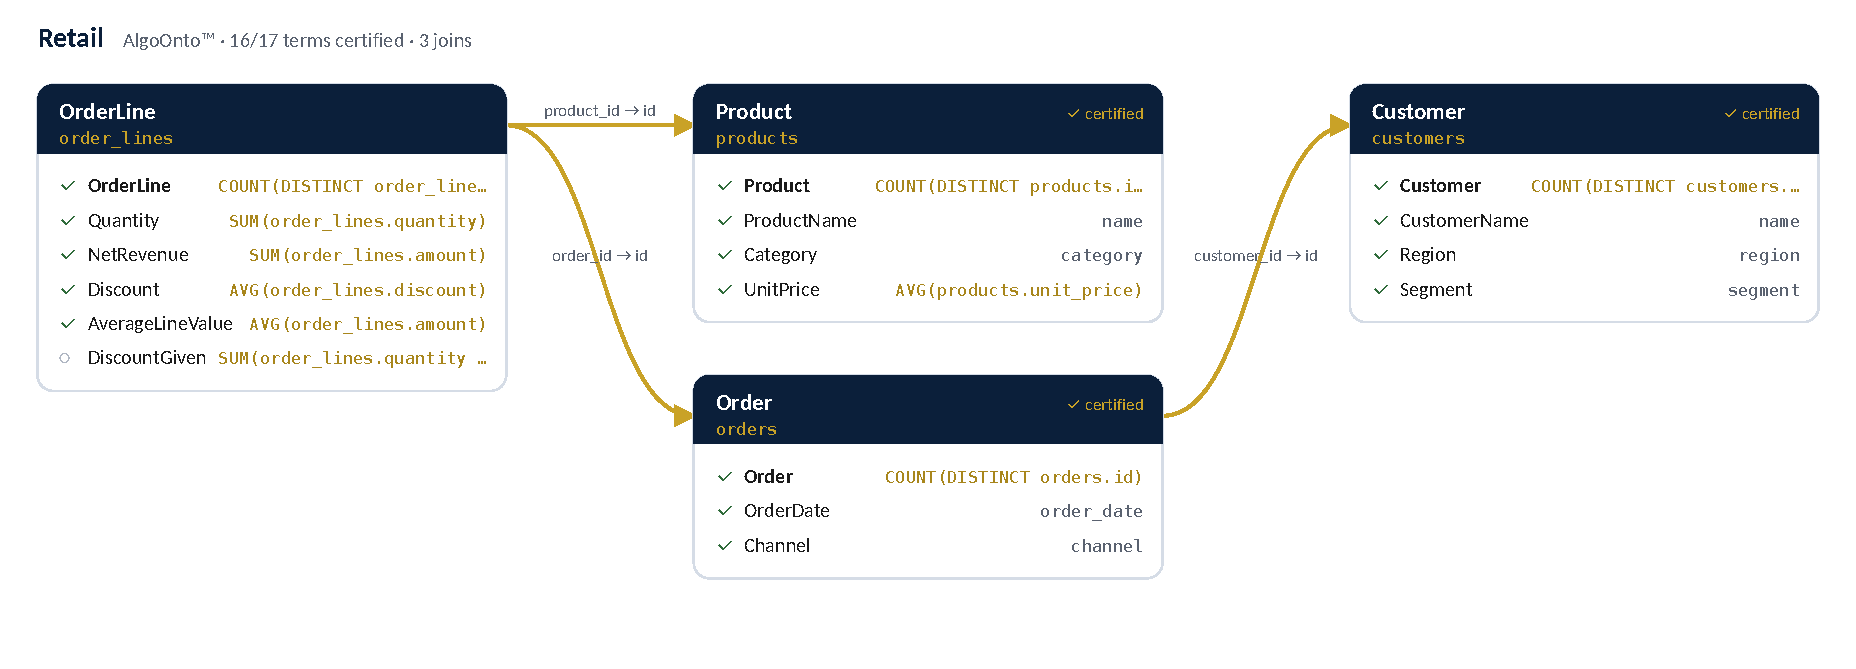
\includegraphics[width=\linewidth]{images/algoonto-graph.pdf}
\end{center}

\section{One ontology, three engines}

An ontology's \code{from} names its data source:

\begin{center}\small
\begin{tabularx}{\linewidth}{@{}lX@{}}
\toprule
\textbf{Source} & \textbf{Opened as} \\
\midrule
\code{"retail.db"} & SQLite file, \code{mode=ro}, with a progress-handler time limit \\
\code{"duckdb:retail.duckdb"} & DuckDB file, \code{read\_only}, with an interrupt timer \\
\code{"postgresql://analyst@host/retail"} & PostgreSQL, in a read-only transaction with \code{statement\_timeout}; client encoding UTF-8 \\
\bottomrule
\end{tabularx}
\end{center}

Discovery, checking, planning, validation, answering and drift all go through one read-only source layer, so no planned query and no validated SQL can change data or run for ever. Each engine's catalogue is read in its own way (SQLite pragmas, DuckDB's constraint tables, PostgreSQL's information schema), and year filters use each engine's own date function. The same questions give the same answers on all three engines; the test suite checks this against a PostgreSQL 16 server in continuous integration. DuckDB and PostgreSQL need \code{pip install "algolang[data]"}.

\paragraph{No passwords in code.} Credentials come from the environment (\code{PGUSER}, \code{PGPASSWORD}) or from \code{\$\{VAR\}} references in the source string. When discovery is given a connection string with a password, it writes \code{\$\{PGPASSWORD\}} in place of the password, and the compiler rejects an ontology whose source contains one (\errcode{E136}).

\section{Drift}

Definitions are certified against the data as it was. \code{algo onto snapshot} records that baseline: every table's columns, types and row count, the values of categorical columns (at most 50 distinct values, and at most one per two rows), and every measure's value. The snapshot is kept next to the ontology and reviewed with it. \code{algo onto drift} compares the data now with the snapshot:

\begin{center}\small
\begin{tabularx}{\linewidth}{@{}lX@{}}
\toprule
\textbf{Severity} & \textbf{Finding} \\
\midrule
breaking & a mapped table or column removed (with a ``renamed?'' hint naming new columns), a type change, a measure that no longer runs \\
warning & a category gained or lost values (a new region, a new channel); a table's rows or a measure's value moved by more than \code{--tolerance} (default 25\%) \\
info & tables and columns the ontology does not cover yet: candidates for new terms \\
review & every certified term touched by a breaking change or a warning: its certification should be renewed \\
\bottomrule
\end{tabularx}
\end{center}

The command exits with status 1 on a breaking change, and also on warnings with \code{--strict}, so it can run on a schedule or in a pipeline before agents rely on the definitions.

\section{Standard exports}

\code{algo onto export --format ttl} (or \code{owl}) writes OWL/RDF in Turtle; \code{--format jsonld} writes JSON-LD; both describe the same graph. Entity terms (a term whose measure counts its table's key) become \code{owl:Class}; other terms become \code{owl:DatatypeProperty} whose \code{rdfs:domain} is their table's entity; declared joins become \code{owl:ObjectProperty}. Synonyms are \code{skos:altLabel}, descriptions \code{skos:definition}. Columns, measures, joins and certification (\code{certifiedBy}, \code{certifiedOn}, \code{status}) use the \code{algo:} vocabulary. Term IRIs default to \code{urn:algolang:onto:<Name>\#<Term>}; \code{--base} sets another.

\section{Graph view}

\code{algo onto graph --html} draws an ontology as a web page, and Studio's \textbf{AlgoOnto\texttrademark} page (\code{/ontology}) draws every ontology in the workspace. Each table is a card with its entity and terms; certified measures are shown in gold; a tick marks a certified term and a circle a proposed one; cards are laid out left to right along the declared joins, which are drawn as labelled arrows.
